\documentclass[fleqn,10pt]{physiome}
% \usepackage[colorlinks,pdfstartview=FitH,citecolor=blue,linkcolor=blue,urlcolor=blue]{hyperref}
\usepackage{caption}
\usepackage{subcaption}
\newcommand{\pluseq}{\mathrel{+}=}
\newcommand{\minuseq}{\mathrel{-}=}
\newcommand{\asteq}{\mathrel{*}=}
\newcommand{\diveq}{\mathrel{/}=}

\articletype{Original}
%% Choose from Original, Retrospective, Review, Letter

\title{A kinetic model of $\beta$-adrenergic control in cardiac myocytes}

\author[1][s.fong@auckland.ac.nz]{Shelley Fong}
\author[2]{Jeffrey J. Saucerman}
\affil[1]{Auckland Bioengineering Institute, The University of Auckland, New Zealand}
\affil[2]{Biomedical Engineering, The University of Virginia, USA}

%% The following lines can be omitted when submitting;
%% information will be added by editors
\publicationdate{23 Sept 2021}
\editor{David P. Nickerson}
\curator{Weiwei Ai}
\submitteddate{3 Sept 2021}
\accepteddate{23 Sept 2021}
\citethisas{Fong and Saucerman (2021)\\A kinetic model of beta-adrenergic control in cardiac myocytes. Physiome.}{10.36903/physiome.16664248}
\begin{document}

\maketitle

\begin{abstract}
The system of equations and figures presented in \cite{saucerman2003} are verified and reproduced in this paper's curation effort. These checks are performed in MATLAB. With some parameter additions and modifications, we can reproduce all figures with small mismatches.
\end{abstract}

\keywords{$\beta$-adrenergic, cardiac myocyte, MATLAB}

\primarypubs[10.36903/physiome.16664248]{refs}{saucerman2003}


\section{Introduction}

$\beta$-adrenergic signalling within the cardiac myocyte is a well-documented signalling pathway, but few mathematical models exist of the complete system. \cite{saucerman2003} published such a model of the activation of the signalling cascade from a ligand  binding the receptor on the cell surface, to triggering the activation of the beta-1 adrenergic receptor ($\beta$1AR), cyclic AMP (cAMP), adenylyl cyclase (AC), protein kinase A (PKA), and phospholamban (PLB). Subsequent downstream effects on ion channel activity are the result, notably through modifying the activity of calcium channels in the regulation of an action potential.

This present work involves the mathematical curation the model.
MATLAB \citep{MATLAB:2017} code was obtained from the first author of \cite{saucerman2003} in an effort to reproduce the figures of that paper. While there is not an exact correspondence between equations presented in the paper and code provided, the figure trends are still reproduced, and numeric values are matched with some modifications/additions made to parameter values, as detailed in under Model Modifications.

A persistent workspace of the code is available in the Physiome Model Repository, at 
 \url{https://models.physiomeproject.org/workspace/6fa}.\\
This workspace includes the MATLAB source code for running the model. The corresponding CellML \citep{cuellar} implementation is available at \url{https://models.physiomeproject.org/e/6f6} which contains the encoding of the mathematics, but does not reproduce the figures due to limited solver capabilities at time of testing. As such, we have elected to do this present curation in MATLAB.

\section{Model description}

The model is broken into several modules:
\begin{itemize}
    \item $\beta$1AR activation
    \item Gs protein activation
    \item cAMP metabolism
    \item PKA activation
    \item PLB regulation 
    \item L-type calcium channel (LCC) regulation 
\end{itemize}

Once the cell is activated by an agonist isoproterenol (Iso), the collective effects of these modules are studied downstream. This includes changes to ion channel activity towards the production and management of an action potential.


\section{Model Modifications}

\subsection{Mathematical Equations}
These are the same as reported in the supplementary material of \cite{saucerman2003} with the exception of the L-type calcium channel. 
This is a reduced-state version of the original model by \cite{jafri1998}, which was implemented in the MATLAB code provided by the original author. The version of the model published in \cite{saucerman2003} showed a complete version of the model as in \cite{jafri1998}, replicated to represent phosphorylated states.

\subsection{Parameter Values}
The baseline parameter values are provided in the supplementary material of \cite{saucerman2003} and in the MATLAB code provided by Saucerman. Missing values on cell geometry are provided in \autoref{tab:parameterMods} which are used in all Figure reproductions. 
\begin{table}[h]
    \centering
    \begin{tabular}{|l|l|l|}
    \hline
    Name & Value & Source\\
    \hline
    Myocyte volume & $36.8\ pL$ & \cite{bers2001}\\
    Myocyte density & $1.06\ g/mL$ & \cite{mendez1960}\\
    \hline
    \end{tabular}
    \caption{Parameters sourced for the model, which were not included in the primary paper.}
    \label{tab:parameterMods}
\end{table}

It was found that the density of myocytes needed to increase by 6.4 times in order to better match the primary paper figures.

\iffalse
    \begin{table}[]
        \centering
    \begin{tabular}{|l|l|l|}
    \hline
    Parameter & Value & Unit \\ 
    \hline
    [Iso] & 0 & $\mu M$ \\ 
    $[IBMX_{tot}]$ & 0 & $\mu M$ \\ 
    $[Fsk_{tot}$] & 0 & $\mu M$ \\ 
    $K_{Gs\alpha }$ & 0.4 & $\mu M$ \\ 
    $K_{AC,FSK}$ & 7.3 & $\frac{1}{s}$ \\ 
    $K_{m,PDE}$ & 1.3 & $\mu M$ \\ 
    $K_{FSK}$ & 44 & $\mu M$ \\ 
    V$_{myo}$ & 20.8 & $\mu L$ \\ 
    V$_{NSR}$ & 9.88e-7 & $\mu L$ \\ 
    V$_{JSR}$ & 9.3e-8 & $\mu L$ \\ 
    A$_{cap}$ & 1.534e-4 & cm$^2$ \\ 
    T & 310 & K \\ 
    $[Na]_e$ & 140 & $mM$ \\ 
    $[K]_e$ & 5.4 & $mM$ \\ 
    $[Ca]_e$ & 1.8 & $mM$ \\ 
    $G_{Na}$ & 8 & $\frac{mS}{\mu F}$ \\ 
    $G_{to}$ & 0.35 & $\frac{mS}{\mu F}$ \\ 
    $G_{ss}$ & 0.07 & $\frac{mS}{\mu F}$ \\ 
    $G_{\bar{ki}}$ & 0.24 & $\frac{mS}{\mu F}$ \\ 
    $G_{kp}$ & 0.008 & $\frac{mS}{\mu F}$ \\ 
    f$_{nLCC}$ & 300 & $\frac{1}{s}$ \\ 
    $\gamma_{o,LCC}$ & 5187.5 & $\frac{1}{mM.s}$ \\ 
    p$_{Ca}$ & 1.7469e-8 & $\frac{cm}{s}$ \\ 
    p$_{K}$ & 3.234e-11 & $\frac{cm}{s}$ \\ 
    N$_{LCC}$ & 3e5 & $\frac{N}{cells}$ \\ 
    I$_{Ca05}$ & -0.458 & $\frac{\mu A}{\mu F}$ \\ 
    $K_{NaCa}$ & 1483 & $\frac{\mu A}{\mu F}$ \\ 
    $K_{Na}$ & 87.5 & $mM$ \\ 
    $K_{Ca}$& 1.38 & $mM$ \\ 
    $k_{sat}$ & 0.1 & 1 \\ 
    $\eta$ & 0.35 & 1 \\ 
    $i_{\bar{NaK}}$ & 1.1 & $\frac{\mu A}{\mu F}$ \\ 
    $K_{m,Na_i}$ & 10 & $mM$ \\ 
    $K_{m,Ko}$ & 1.5 & $mM$ \\ 
    $i_{\bar{PCa}}$ & 1.15 & $\frac{\mu A}{\mu F}$ \\ 
    $K_{m,pCa}$ & 5e-4 & $mM$ \\ 
    $G_{CaB}$ & 2.8e-3 & $\frac{\mu A}{\mu F}$ \\ 
    $G_{NaB}$ & 1.18e-3 & $\frac{\mu A}{\mu F}$ \\ 
    $I_{\bar{up}}$ & 4.7 & $\frac{mM}{s}$ \\ 
    $K_{m,Up}$ & 3e-4 & $mM$ \\ 
    $\bar{NSR}$ & 15 & $mM$ \\ 
    $\tau_{on}$ & 2e-3 & $s$ \\ 
    $\tau_{off}$ & 2e-3 & $s$ \\ 
    $g_{max,rel}$ & 60e3 & $\frac{mM}{s}$ \\ 
    $\bar{CSQN}$ & 15 & $mM$ \\ 
    $K_{m,CSQN}$ & 0.8 & $mM$ \\ 
    $\tau_{tr}$ & 5.7e-4 & $s$ \\ 
    $\bar{TRPN}$ & 0.07 & $mM$ \\ 
    $\bar{CMDN}$ & 0.05 & $mM$ \\ 
    $\bar{INDO}$ & 0.07 & $mM$ \\ 
    $K_{m,TRPN}$ & 0.5128e-3 & $mM$ \\ 
    $K_{m,CMDN}$ & 2.38e-3 & $mM$ \\ 
    $K_{m,INDO}$ & 8.44e-4 & $mM$ \\ 
    \hline
    \end{tabular}
        \caption{Caption}
        \label{tab:my_label}
    \end{table}
\fi

\begin{table}
\begin{tabular}{|l|l|l|l|}
\hline
Figure & Parameter values & Number of iterations & T (min)  \\ 
\hline
2a &  & 1 & 18 \\ 
\hline
2b & $[Iso^\dagger] = \texttt{logspace(-3,0.45,8)}\ \mu M$ & & 6 \\ 
 & $[IBMX] = 100\ \mu M$ & 8 & \\ 
\hline
2c, 2d & $[Iso] = 1\ \mu M$ & 6 & 1 \\ 
 & $[[PKI] = \{0, 0.052\}\ \mu M$ & & \\
 & $[cAMP^\dagger] = \texttt{logspace(-1.9,2,6)}\ \mu M$ & & \\
\hline
2e & $[Iso^\dagger] = \texttt{logspace(-6,0,20)}\ \mu M$ & 20 & 30 \\ \hline
2f & $[Iso^\dagger] = \{0, 1\}\ \mu M$ & 2 & 1 \\
\hline
2g, 2h & $[Iso^\dagger] = \{0, 1\}\ \mu M$ & 2 & 1 \\
\hline
3a & $[Iso^\dagger] = \texttt{logspace(-3,0,8)}\ \mu M$ & 32 & 7 \\
& $[AC]_{tot} \asteq 3$  &  & \\
 &  $[\beta1AR_{tot}] \asteq 3$  &  & \\
 &  $K_{Gs\alpha } \diveq 3$ &  & \\
\hline
3b & $[Iso^\dagger] = \texttt{logspace(-3,0,8)}\ \mu M$ & 32 & 7 \\
& $[AC]_{tot}\ \asteq 1.5$  & & \\
 &  $[\beta1AR_{tot}]\ \asteq 1.8$  & & \\
 &  $K_{Gs\alpha }\ \diveq 1.9$ & & \\
\hline
4a, 4b & $[IBMX] = 250\ \mu M$ & 3 & 3 \\
& $[Iso^\dagger] = \{1,0,1\}\ \mu M$ &  &  \\
& $k_{hyd}^\dagger\ \asteq \{1,0.05,0.05\} $ &  &  \\
\hline
5 & $[Iso^\dagger] = \texttt{logspace(-4,0,8)}\ \mu M$ & 24 & 20 \\
& $[PKA_{I,tot}]\ \asteq0.05$ & & \\
& $[PKI_{tot}]\ \asteq0.05$ & & \\
\hline
6a & $[Iso^\dagger] = \{1,1,1\}\ \mu M$ & 3 & 1 \\
& $[PLBp^\dagger]^{t=0} \ \asteq \{1,0,1\}$ & & \\
& $[LCCap^\dagger]^{t=0} \ \asteq \{1,0,1\}$ & & \\
& $[LCCbp^\dagger]^{t=0} \ \asteq \{1,0,1\}$ & & \\
\hline
6b & $[Iso^\dagger] = \{0,1,0,1\}\ \mu M$ & 4 & 1 \\
 & fracPLB$^\dagger\ \asteq \{1,1,0,0\}$ & & \\
 & fracPLBo$^\dagger\ \asteq \{1,1,0,0\}$ & & \\
\hline
\end{tabular}
\caption{Specific protocol followed in the reproduction of each figure, run for a span of T minutes. $\asteq, \diveq$ indicate multiplication or division of parameter by the specified value respectively. $\dagger$ denotes the variable value being changed with every iteration. One iteration constitutes running the entire model once. For multiple species being changed for one figure: for the $n$th loop iteration, the value of the species is given by the $n$th value in the sequence given in the sequence (Column 2) for all marked species. (3a, 3b): four separate iterations for every [Iso]: one control, one with changed $[AC_{tot}]$ only, one with changed $[\beta1AR_{tot}]$ only, and one with change $K_{Gs\alpha }$ only. (5): three separate iterations for every [Iso]: one control, one with changed $[PKA_{I,tot}]$ only, one with changed $[PKI_{tot}]$ only. patch clamping: Figures 2g-h, 6b follow Protocol 1; Figure 2f follows Protocol 2 (see \autoref{tab:vprotocol}).\\ 
See primary paper or source code for an explanation of all chemical abbreviations.}
\label{tab:figureConditions}
\end{table}

\begin{table}
    \centering
    \begin{tabular}{|p{0.1\textwidth}|p{0.75\textwidth}|} 
    \hline
        Protocol & Details \\
        \hline
        1  & \[ I_{app} =
  \begin{cases}
    10\ \frac{\mu A}{\mu F}  & \  \text{if } \texttt{mod}(t+0.9, 1) <= 5e-3\\
    0\ \frac{\mu A}{\mu F}  & \  \text{otherwise}
  \end{cases}
\] \\
\hline
        2  & \[ V_{clamp} =
  \begin{cases}
    -10\ mV  & \  \text{if } 59.1<t<59.5\\
    -55\ mV  & \  \text{otherwise }
  \end{cases}
\] \\
         & where $I_{app} = \frac{V_{clamp}-V_m}{R_{clamp}}$ \\
         \hline
    \end{tabular}
    \caption{Patch clamp protocols. $R_{clamp} = 0.02\ \Omega$}
    \label{tab:vprotocol}
\end{table}
Experimental conditions specific to each Figure are given in \autoref{tab:figureConditions}. For Figures 2f-h and 6b, patch clamp protocols are defined in \autoref{tab:vprotocol}.

\iffalse
    \subsection{Initial conditions}
    \begin{table}[ht]\centering
    \caption{Initial conditions.}\label{tab:ICs}
    \begin{tabular}{|l|l|l|l|}
    \hline
    index & Variable & Value & Unit \\ 
    \hline
    1  & [L] & 0.01 & $\mu M$ \\ 
    2  & [R] & 0.01079 & $\mu M$ \\ 
    3  & [G] & 3.829 & $\mu M$ \\ 
    4  & [$\beta$1AR$_{tot}$] & 0.01205 & $\mu M$ \\ 
    5  & [$\beta$1AR$_d$] & 0 & $\mu M$ \\ 
    6  & [$\beta$1AR$_p$] & 1.154e-3 & $\mu M$ \\ 
    7  & [GsGTP$_{tot}$] & 0.02505 & $\mu M$ \\ 
    8  & [$Gs\alpha GDP$] & 6.446e-4 & $\mu M$ \\ 
    9  & [$Gs\beta\gamma$] & 0.02569 & $\mu M$ \\ 
    10 & [$Gs\alpha GTP$] & 0.02441 & $\mu M$ \\ 
    11 & [Fsk] & 0 & $\mu M$ \\ 
    12 & [AC] & 0.04706 & $\mu M$ \\ 
    13 & [PDE] & 0.0389 & $\mu M$ \\ 
    14 & [IBMX] & 0 & $\mu M$ \\ 
    15 & [cAMP$_{tot}$] & 0.8453 & $\mu M$ \\ 
    16 & [cAMP] & 0.2268 & $\mu M$ \\ 
    17 & [PKACI] & 0.05868 & $\mu M$ \\ 
    18 & [PKACII] & 8.278e-3 & $\mu M$ \\ 
    19 & [PLB$_p$] & 4.105 & $\mu M$ \\ 
    20 & [Inhib1$_{p,tot}$] & 0.0526 & $\mu M$ \\ 
    21 & [Inhib1$_{p}$] & 6.3e-5 & $\mu M$ \\ 
    22 & [PP1] & 0.838 & $\mu M$ \\ 
    23 & [$LCC_{ap}$] & 5.103e-3 & $\mu M$ \\ 
    24 & [$LCC_{bp}$] & 5.841e-3 & $\mu M$ \\ 
    25 & $m$ & 1.4e-3 & 1 \\ 
    26 & $h$ & 0.99 & 1 \\ 
    27 & $j$ & 0.99 & 1 \\ 
    28 & $v$ & 0 & 1 \\ 
    29 & $w$ & 0 & 1 \\ 
    30 & $x$ & 0.13 & 1 \\ 
    31 & $y$ & 0.96 & 1 \\ 
    32 & $z$ & 0.92 & 1 \\ 
    33 & r$_{to}$ & 1.4e-3 & 1 \\ 
    34 & s$_{to}$ & 1 & 1 \\ 
    35 & ss$_{to}$ & 0.613 & 1 \\ 
    36 & r$_{ss}$ & 198e-3 & 1 \\ 
    37 & s$_{ss}$ & 0.43 & 1 \\ 
    38 & [Ca$_{nsr}$] & 1.92 & $mM$ \\ 
    39 & [Ca$_{jsr}$] & 1.92 & $mM$ \\ 
    40 & [Na$_i$] & 16 & $mM$ \\ 
    41 & [K$_i$] & 145 & $mM$ \\ 
    42 & [Ca$_i$] & 1.58e-4 & $mM$ \\ 
    43 & V$_m$ & -85.66 & $mV$\\ 
    44 & $t_{rel}$ & 0.9 & $s$ \\ 
    \hline
    \end{tabular}
    \end{table}
\fi

This system has 44 dependent variables. Unless stated otherwise, all figure reproductions are subject to the same initial conditions (see source code). These values are embedded in the script \texttt{main.m}.

\section{Computational Simulation}

The system of differential-algebraic equations is solved in MATLAB using stiff solver \texttt{ode15s} \citep{shampine1997matlab} with automatic/adaptive time stepping, $RelTol = 1e-6$, $MaxStep = 5e-3$. No further packages are required; any machine with the full ODE suite (which includes \texttt{ode15s} solver) should be able to run all simulations.

Run the script main.m. The user will be prompted to specify the desired figure reproduction: input the appropriate string of format $ia$ where $i$ is the figure number and $a$ is the subfigure letter: for example, $2b$. 

Figures are highly recommended to be reproduced using parallel computing (parpool, >=4 workers) in MATLAB due to the size and stiffness of the code. By default, this is already set up in the script. Otherwise, computations will take up to 30 minutes per figure, on a 2.8 Ghz / 4 core machine running on Windows 10.
Once running, keep parpool open (change parallel preferences: adjust time to automatically shut down pool after appropriate amount of time) such that time is not lost waiting for the pool to start up on every simulation.

\begin{table}[]
    \centering
    \begin{tabular}{|c|c|c|c|}
    \hline
         Figure & Species & Original value & Value modified for MATLAB \\
         \hline
         2b & max([Iso]) & $10\ \mu M$ & $2.8\ \mu M$ \\
         2c/d & [PKI] & $60\ nM$ & $52\ nM$ \\
         2f & Patch clamp voltage & holding $-80\ mV$, step $0\ mV$ & holding $-55\ mV$, step $-10\ mV$\\
         4a & [IBMX] & $1\ mM$ & $250\ \mu M$\\
         4b & max([Iso]) & $10\ \mu M$ & $1\ \mu M$ \\
         5 & PKAI$_{tot}$& 0 & 5\% of baseline\\
           & PKI$_{tot}$& 0 & 5\% of baseline\\
         6a & [Iso] & - & $1\ \mu M$ \\
         6b & [Iso] & - & $1\ \mu M$ \\
            & fracPLB & - & 0 \\
        \hline
    \end{tabular}
    \caption{Modifications made to stated values of primary paper, in the reproduction of the figures.}
    \label{tab:parameterAdjustments}
\end{table}
The original implementation of the model was performed using Berkeley-Madonna software, with a different ODE solver to MATLAB \citep{saucerman2003}. As some simulation values stated in the primary paper resulted in the model being unsolvable in the MATLAB routine, we had to make adjustments as outlined in \autoref{tab:parameterAdjustments}.

\section{Model Results}
We employ Engauge Digitizer software \citep{mark_mitchell_2020_3941227} to extract data from Figures of \cite{saucerman2003} to present alongside results of the present work.

\begin{figure}
    \centering
    \begin{subfigure}[b]{0.49\textwidth}
        \centering
        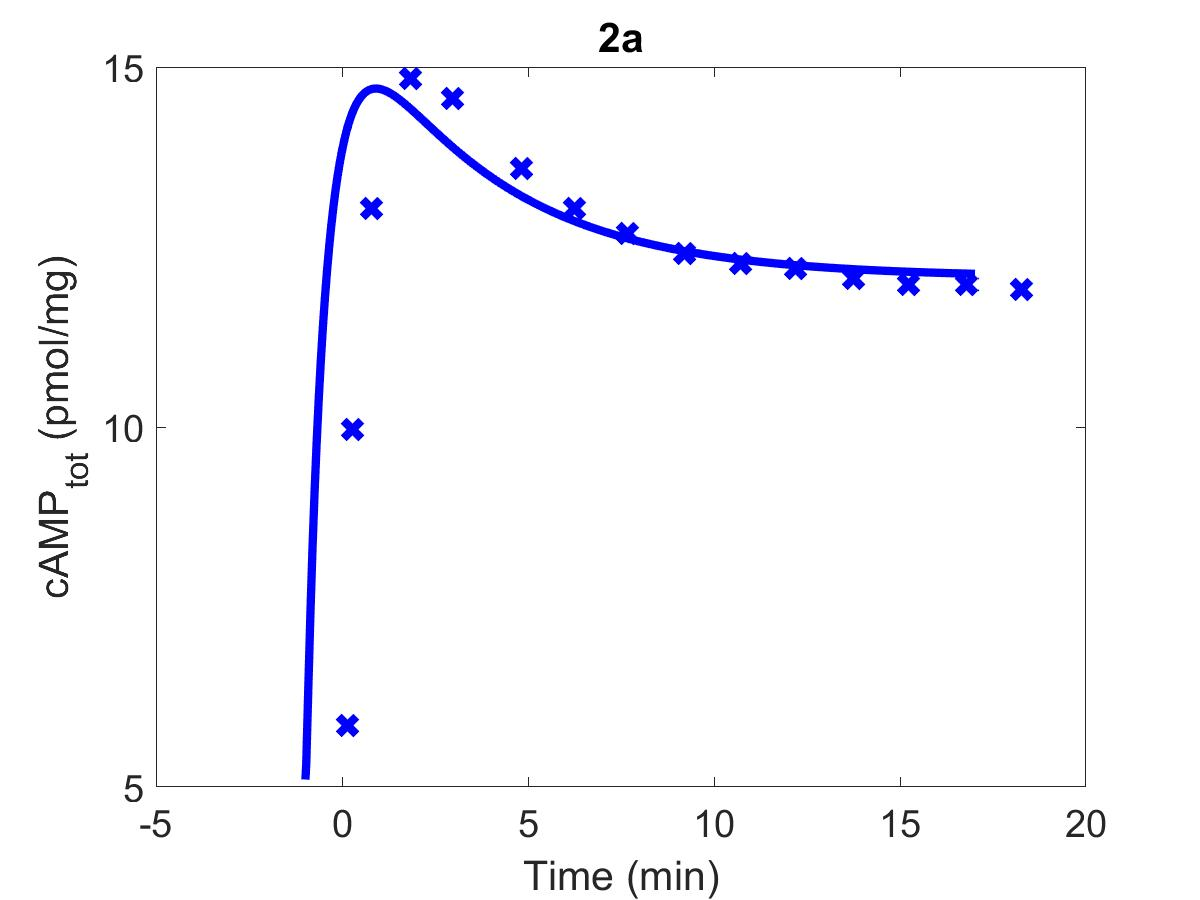
\includegraphics[width=\textwidth]{figures/F2a.jpg}
    \end{subfigure}
    \hfill
    \begin{subfigure}[b]{0.49\textwidth}
        \centering
        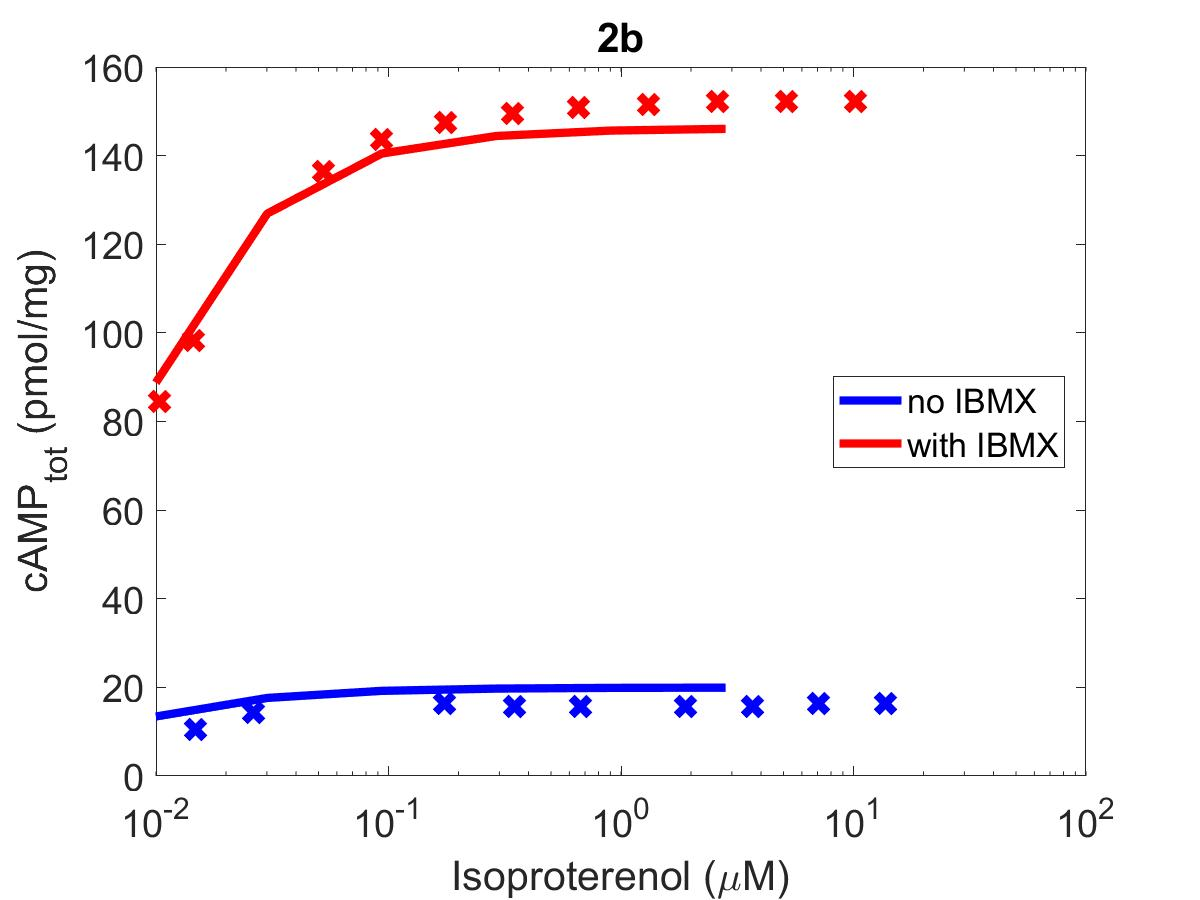
\includegraphics[width=\textwidth]{figures/F2b.jpg}
    \end{subfigure}
    \hfill
    \begin{subfigure}[b]{0.49\textwidth}
        \centering
        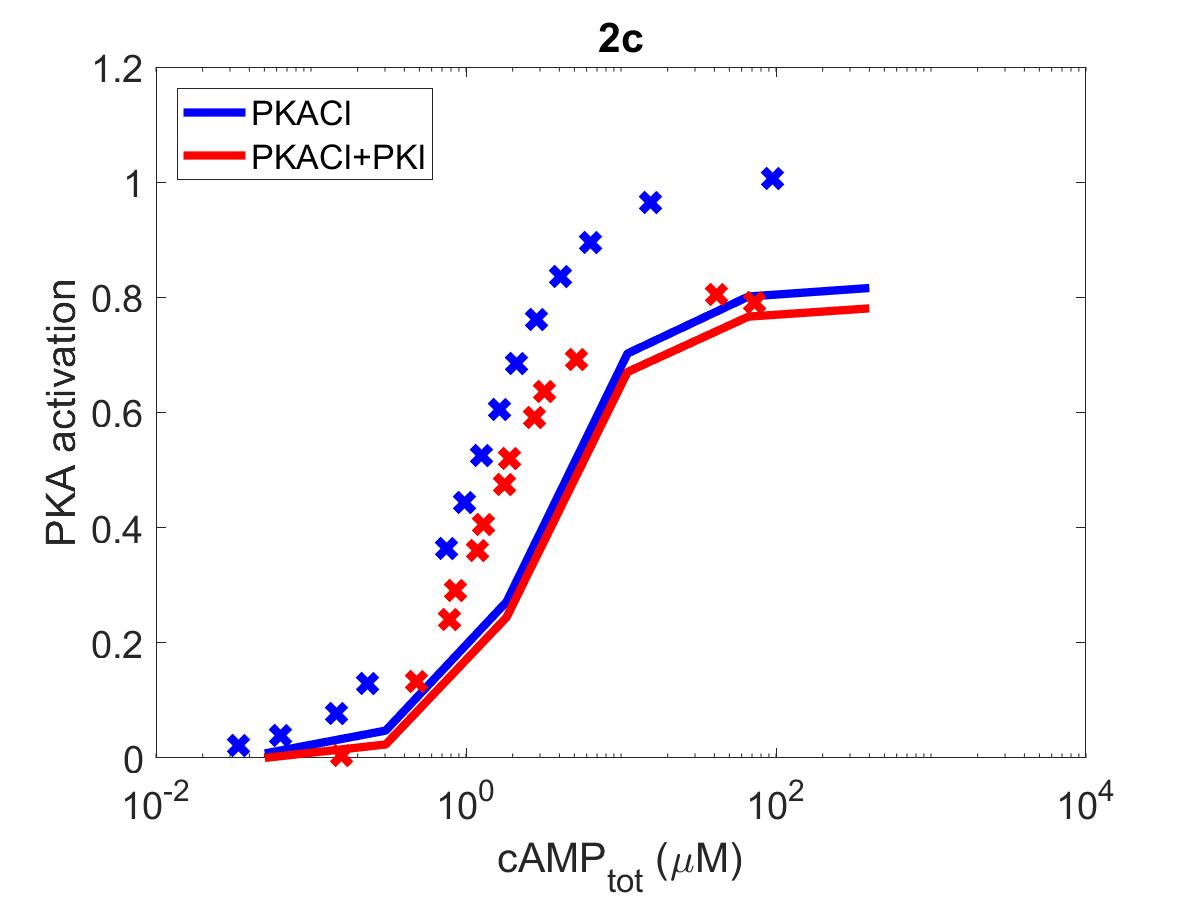
\includegraphics[width=\textwidth]{figures/F2c.jpg}
    \end{subfigure}
    \hfill
    \begin{subfigure}[b]{0.49\textwidth}
        \centering
        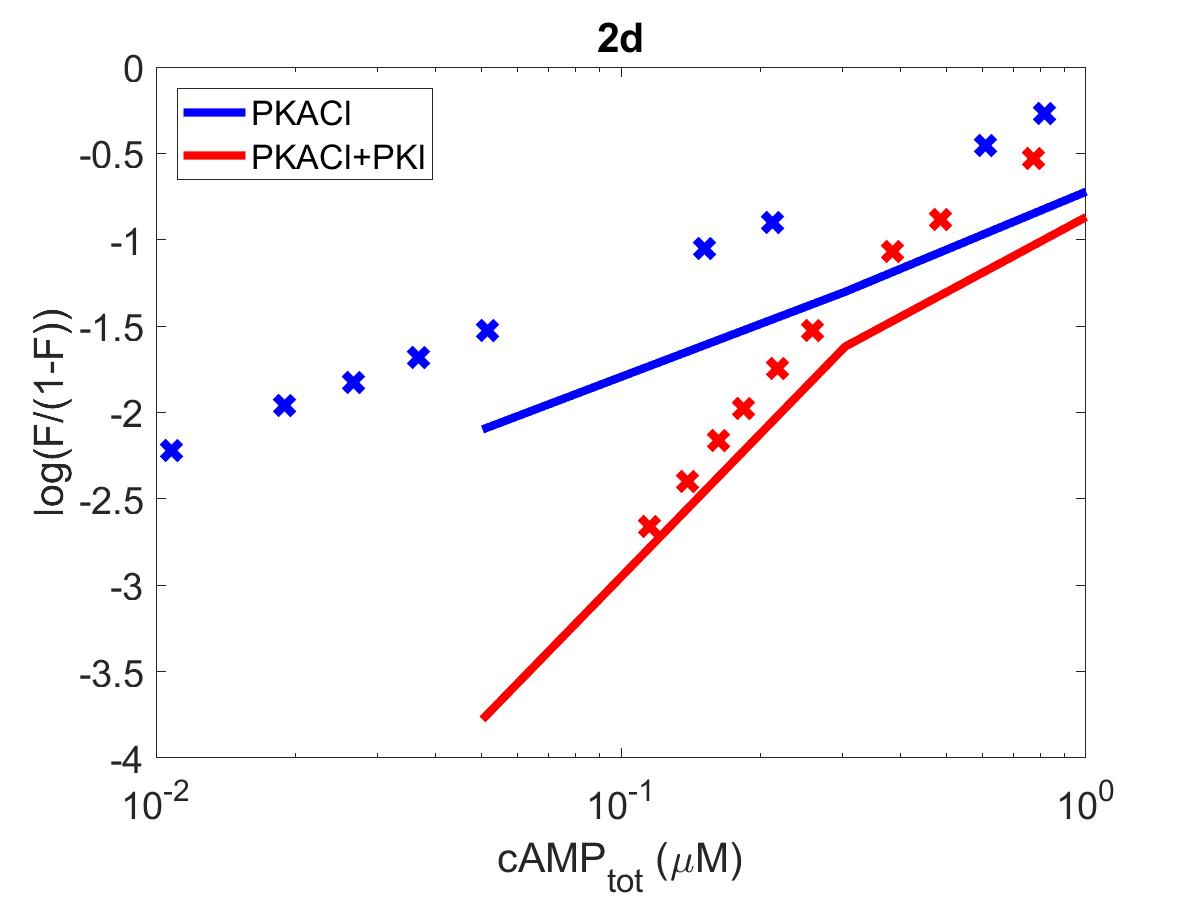
\includegraphics[width=\textwidth]{figures/F2d.jpg}
    \end{subfigure}
    \hfill
    \begin{subfigure}[b]{0.49\textwidth}
        \centering
        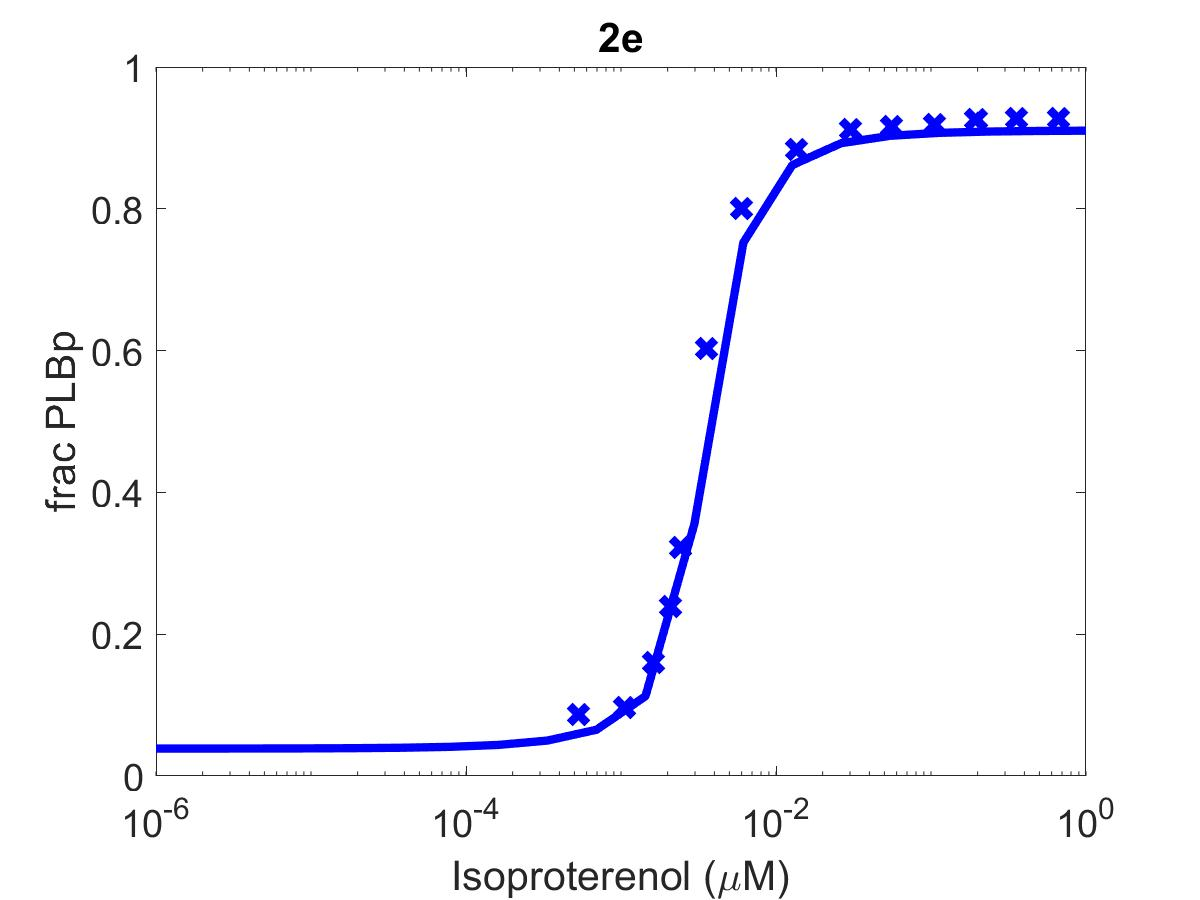
\includegraphics[width=\textwidth]{figures/F2e.jpg}
    \end{subfigure}
    \hfill
    \begin{subfigure}[b]{0.49\textwidth}
        \centering
        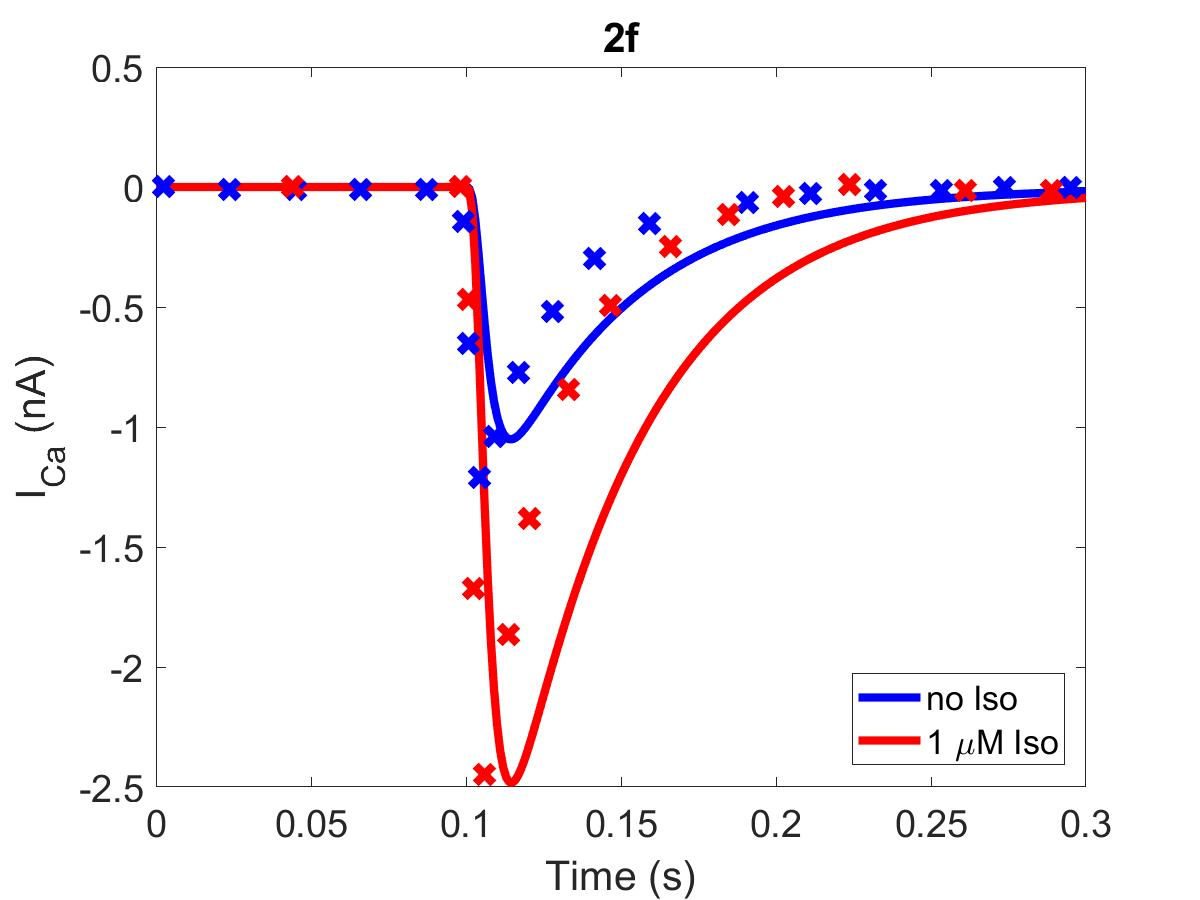
\includegraphics[width=\textwidth]{figures/F2f.jpg}
    \end{subfigure}
    \hfill
    \begin{subfigure}[b]{0.49\textwidth}
        \centering
        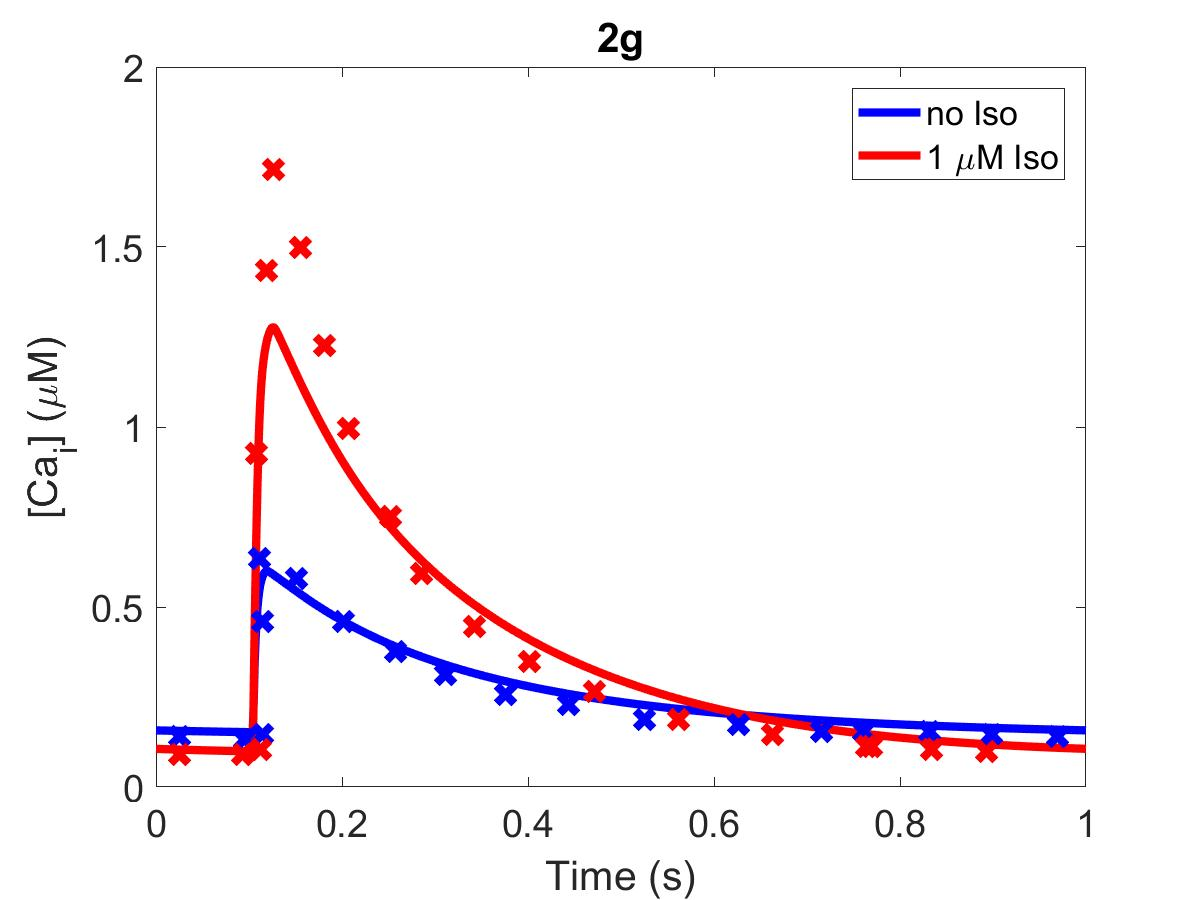
\includegraphics[width=\textwidth]{figures/F2g.jpg}
    \end{subfigure}
    \begin{subfigure}[b]{0.49\textwidth}
        \centering
        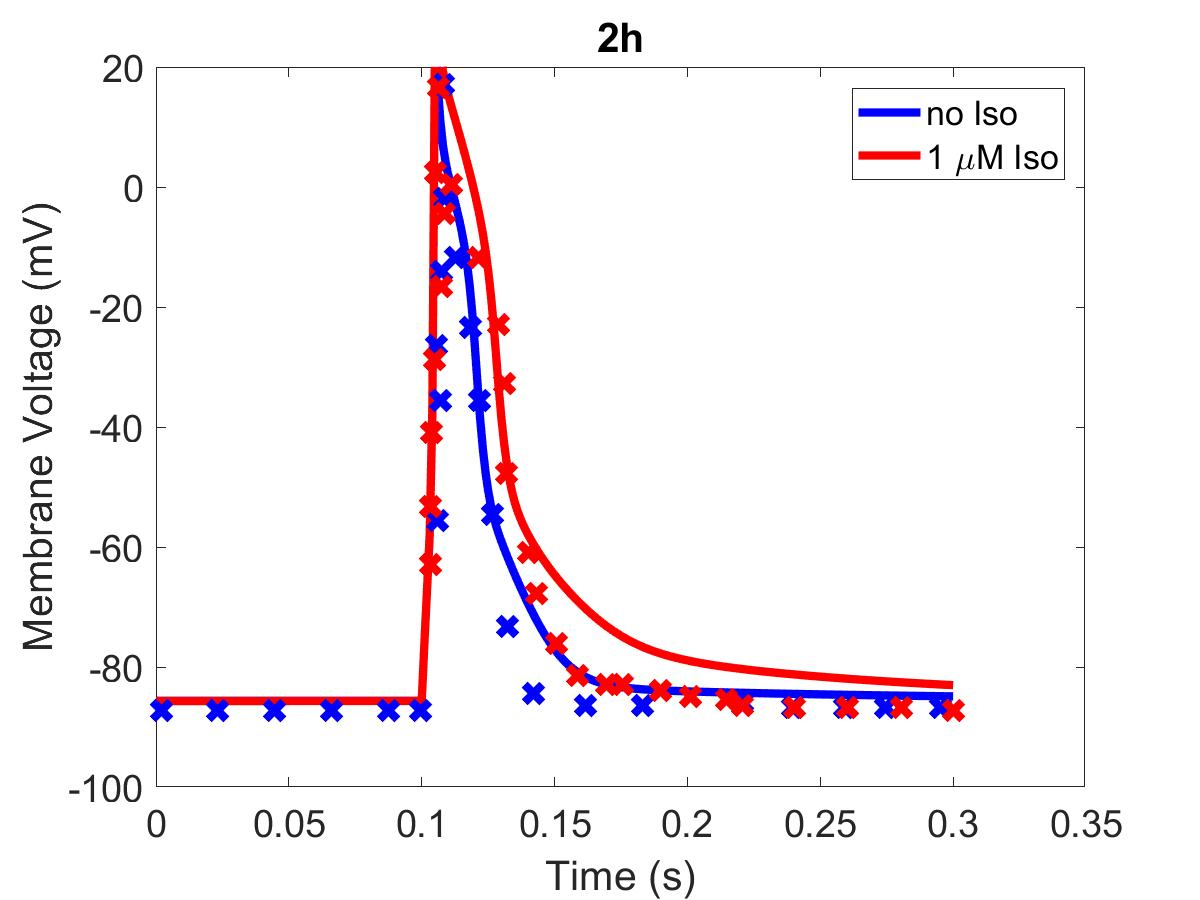
\includegraphics[width=\textwidth]{figures/F2h.jpg}
    \end{subfigure}
    \caption{The primary data ($x$) of Figure 2 with our reproduction of all subfigures ($-$). Note: (2c) $PKA\ activation = \frac{[PKACI]}{2*[PKAI_{tot}]}$}
    \label{fig:2}
\end{figure}


\begin{figure}
    \centering
    \begin{subfigure}[b]{0.49\textwidth}
        \centering
        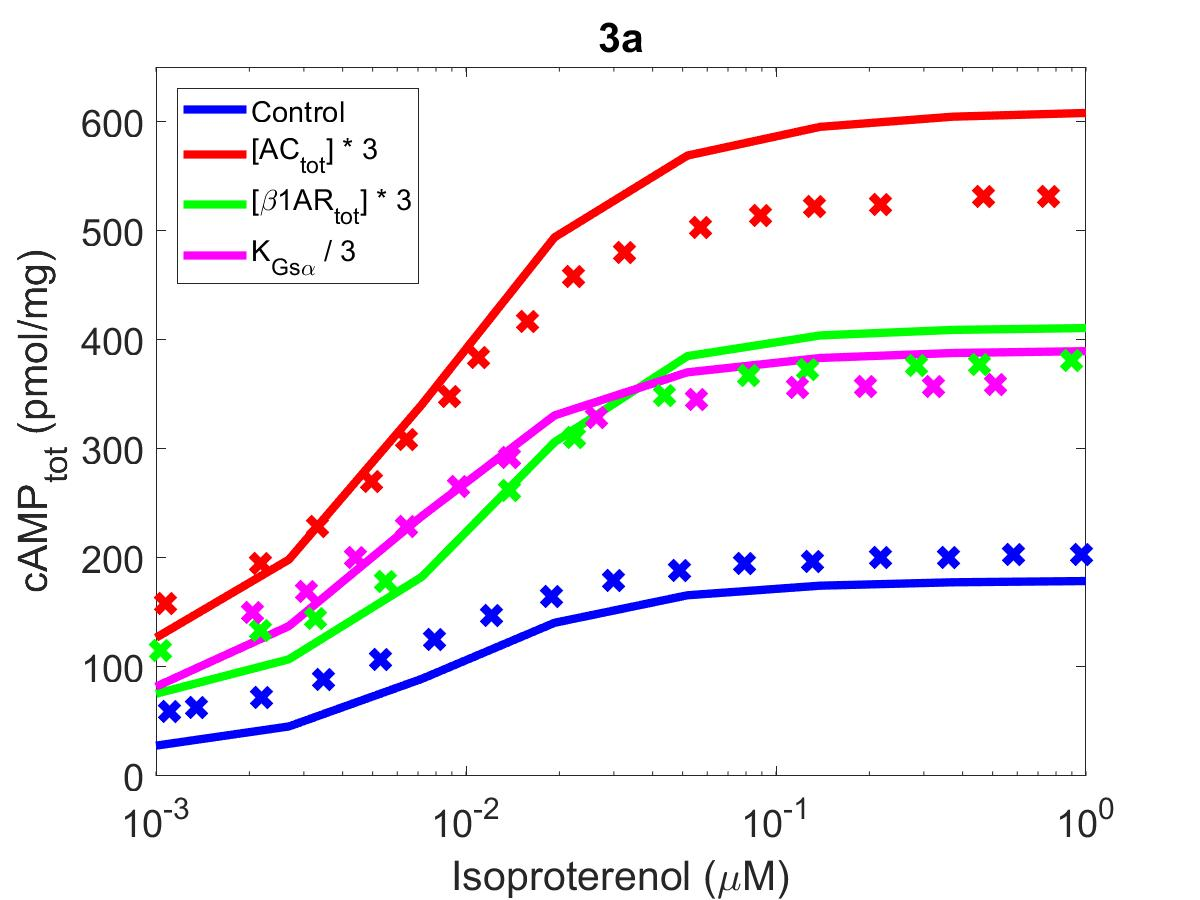
\includegraphics[width=\textwidth]{figures/F3a.jpg}
    \end{subfigure}
    \begin{subfigure}[b]{0.49\textwidth}
        \centering
        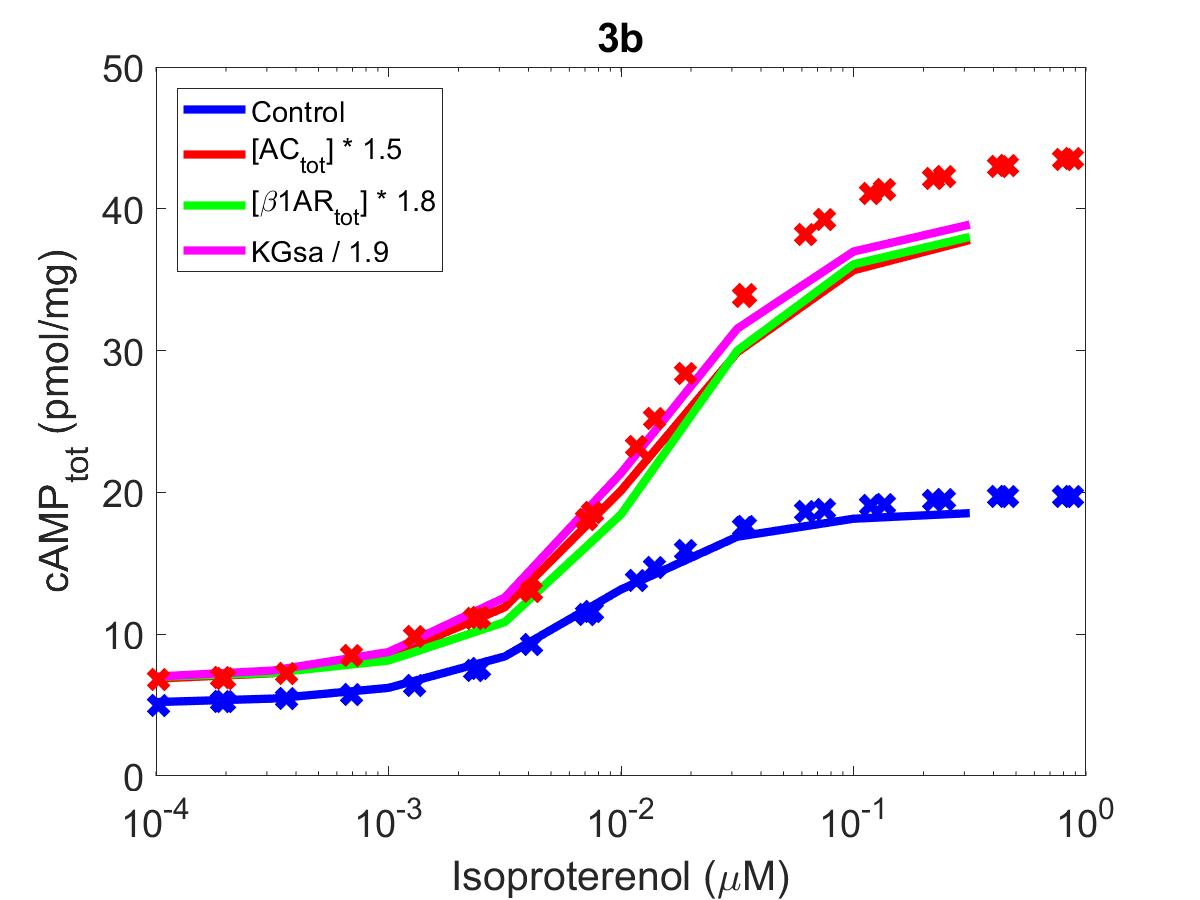
\includegraphics[width=\textwidth]{figures/F3b.jpg}
    \end{subfigure}
    \caption{The primary data ($x$) of Figure 3 with our reproduction of all subfigures ($-$). Note: lines in (3b) showing modifications to $[AC]_{tot}, \beta 1AR, K_{Gs\alpha }$ have been grouped into an average `augmentation' line.}
    \label{fig:3}
\end{figure}

\begin{figure}
    \centering
    \begin{subfigure}[b]{0.49\textwidth}
        \centering
        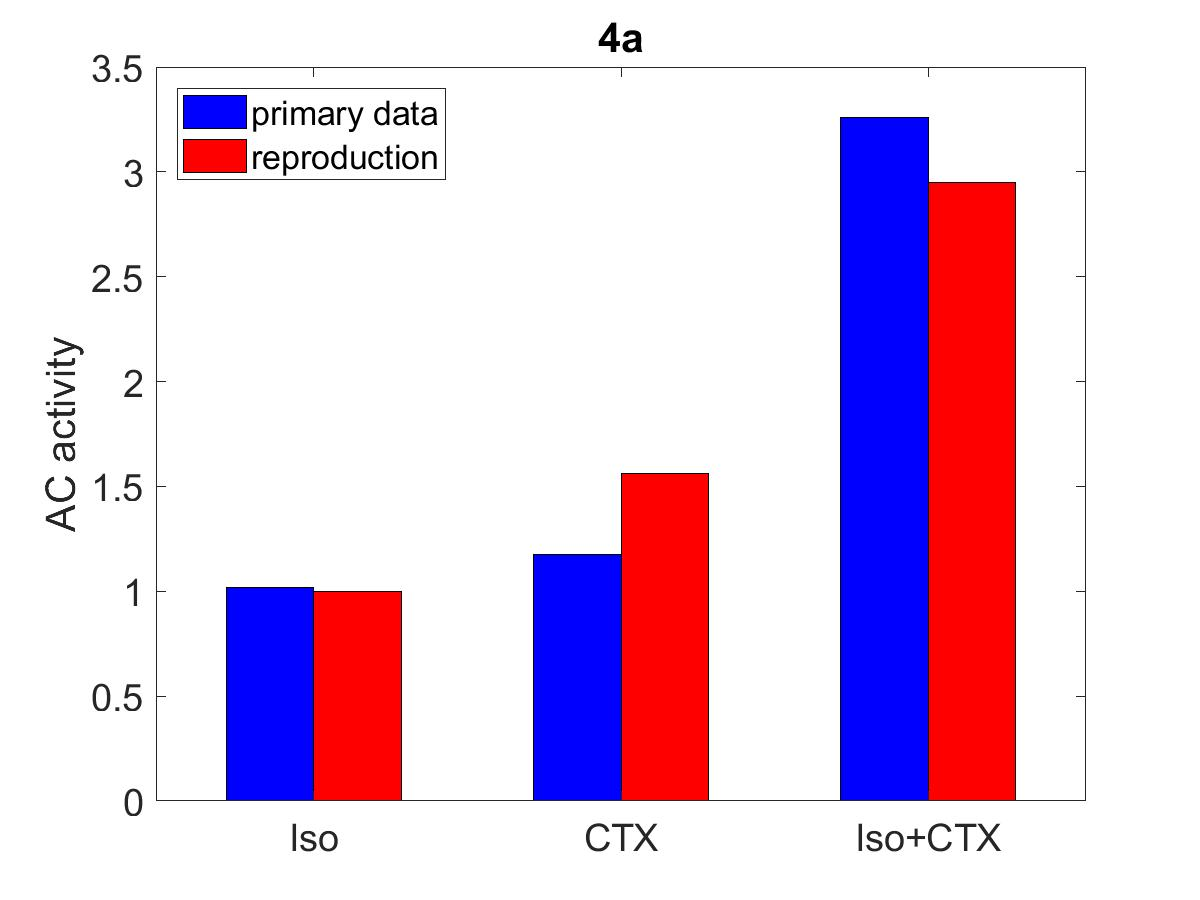
\includegraphics[width=\textwidth]{figures/F4a.jpg}
    \end{subfigure}
    \begin{subfigure}[b]{0.49\textwidth}
        \centering
        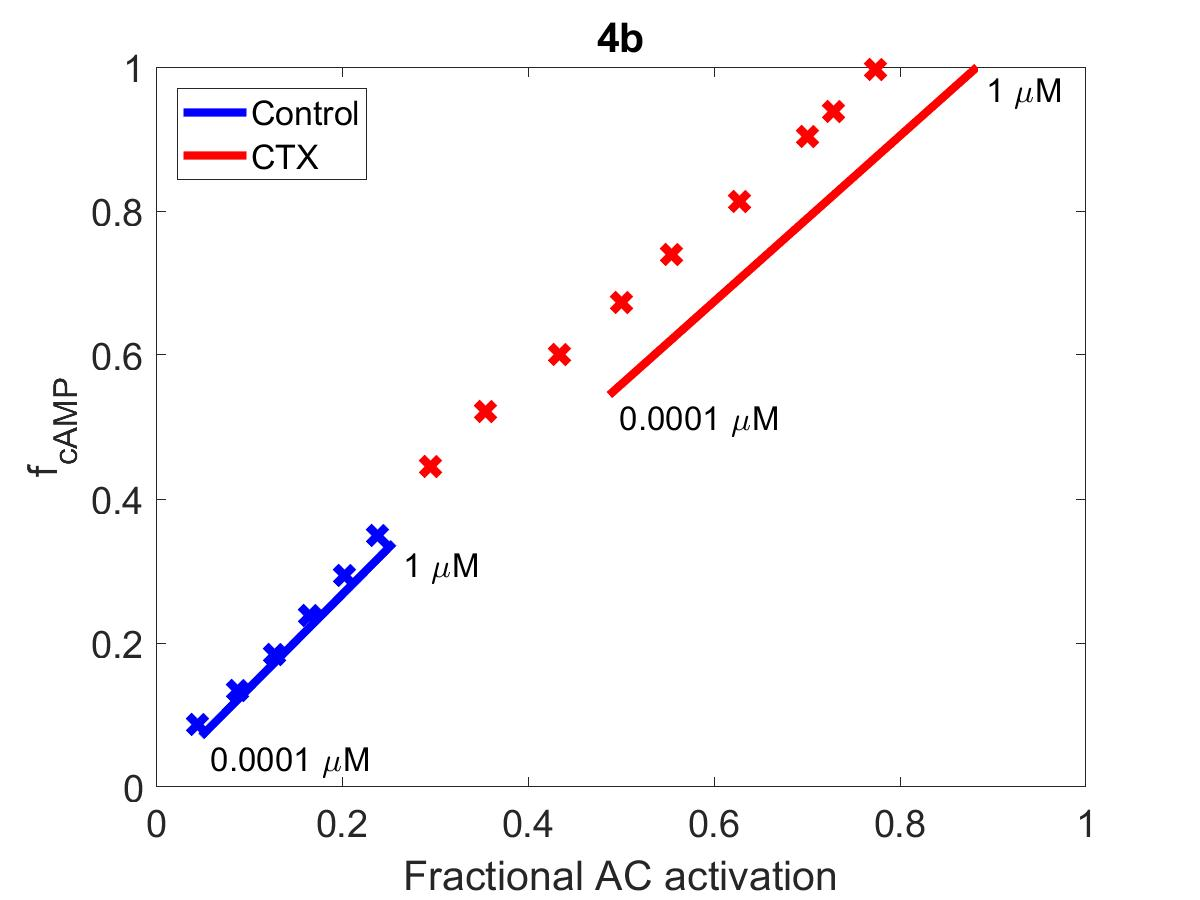
\includegraphics[width=\textwidth]{figures/F4b.jpg}
    \end{subfigure}
    \caption{The primary data ($x$) of Figure 4 with our reproduction of all subfigures ($-$). (4a): primary data shown in blue, reproduction in red. $AC\ activity=cAMP_{tot}$. (4b):  $f_{cAMP}=\frac{cAMP_{tot}}{cAMP_{tot,max}}$. Annotated numbers on the graph refer to [Iso] set for that experiment.}
    \label{fig:4}
\end{figure}

\begin{figure}
    \centering
    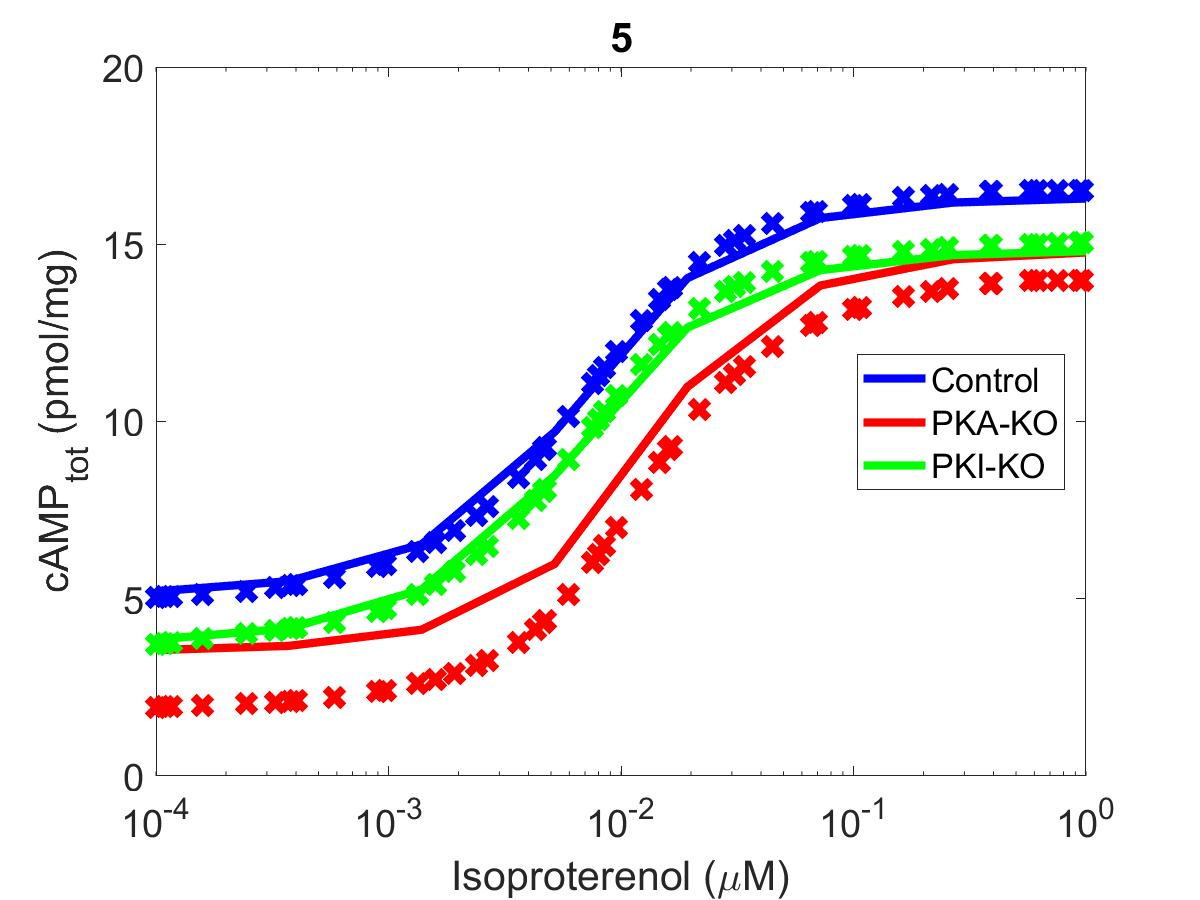
\includegraphics[width=0.49\textwidth]{figures/F5.jpg}
    \caption{The primary data ($x$) of Figure 5 with our reproduction ($-$).}
    \label{fig:5}
\end{figure}

\begin{figure}
    \centering
    \begin{subfigure}[b]{0.49\textwidth}
        \centering
        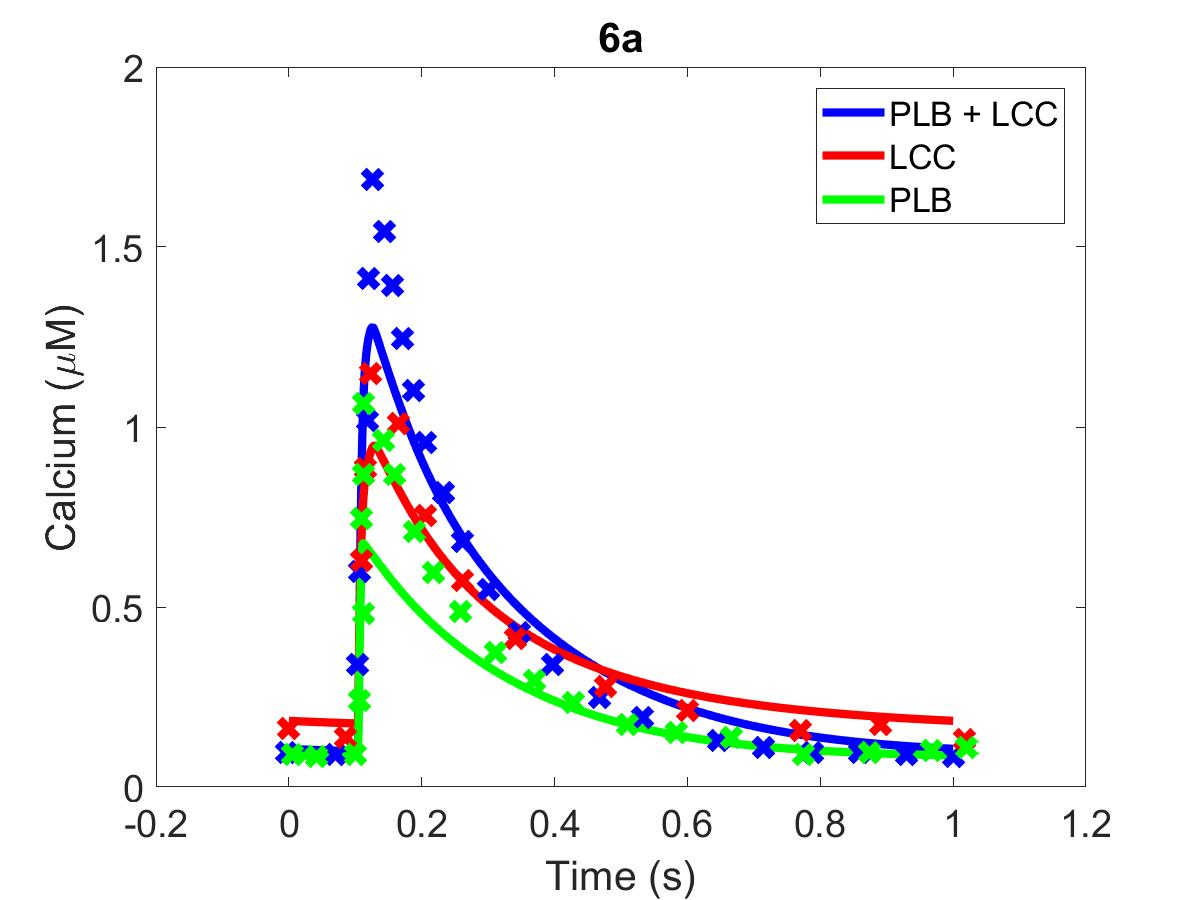
\includegraphics[width=\textwidth]{figures/F6a.jpg}
    \end{subfigure}
    \begin{subfigure}[b]{0.49\textwidth}
        \centering
        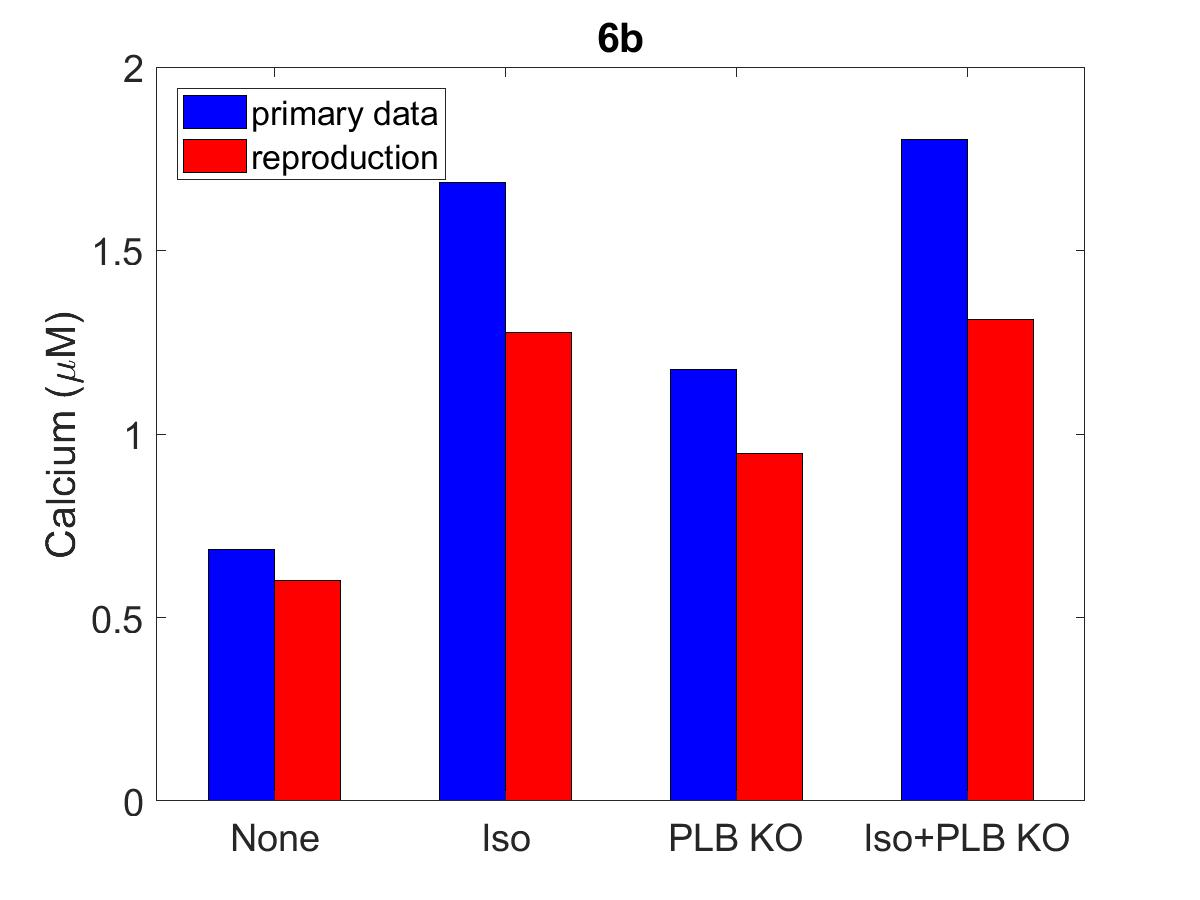
\includegraphics[width=\textwidth]{figures/F6b.jpg}
    \end{subfigure}
    \caption{(6a) The primary data ($x$) of Figure 6a with our reproduction of all subfigures ($-$). (6b) Primary data shown in blue, reproduction in red.}
    \label{fig:6}
\end{figure}

The reproduction of all figures of \cite{saucerman2003} are given in Figures \ref{fig:2}-\ref{fig:6}, which show good agreement against the data of the primary paper. Solid lines show the output from this curation effort, and crosses show discrete points found by the Engauge Digitizer of the figures originally published.

\section{Discussion}

We demonstrate that figures of \cite{saucerman2003} can be reproduced given some additions (\autoref{tab:parameterMods}) and adjustments (\autoref{tab:parameterAdjustments}) made to model parameter values. There are slight deviations of the curated model output from the original data which can be attributed to parameter modifications we had to make to ensure a simulation runs to completion (see Figures 1c, 1d, 3a, 3b). Other mismatches may be owing to differences from the original implementation in Berkeley-Madonna, which had different solver settings to this effort. The original code is no longer available. 

As this paper follows the tenets of FAIR \citep{wilkinson2016fair}, further credibility is lent to the original model. The model has already proven to be valuable to the mathematical modelling community in understanding the workings of $\beta$-adrenergic receptor signalling within cardiac myocytes.


\bibliography{refs}

\end{document}